\documentclass{article} % For LaTeX2e
\usepackage{nips14submit_e,times}
\usepackage{hyperref}
\usepackage{url}
\usepackage{amsmath,amsfonts,amsthm}
\usepackage{bbm}
\usepackage{algorithm,algorithmic}
\usepackage{graphicx}
\usepackage{bm}
\usepackage{bbm}
\usepackage[titletoc]{appendix}
\usepackage{wrapfig}
\usepackage{afterpage}
\usepackage{amssymb}

\def\B#1{\bm{#1}}
%\def\B#1{\mathbf{#1}}
\def\trans{\mathsf{T}}

%\renewcommand{\labelitemi}{--}

\newtheorem{theorem}{Theorem} \newtheorem{lemma}[theorem]{Lemma}
\newtheorem{proposition}[theorem]{Proposition}
\newtheorem{corollary}[theorem]{Corollary}
\newtheorem{definition}[theorem]{Definition}
\newtheorem{remark}{Remark}

%%%%%%%%%%%%%%%%%%%%%%%%%%%%%%%%%%%%%%%%%%%%%%%%%%%%%%%%%%%%%%%%%%%%%%%%%%%%%%%

\title{Semi-supervised low-rank logistic regression for
high-dimensional neuroimaging data}

\newcommand{\fix}{\marginpar{FIX}}
\newcommand{\new}{\marginpar{NEW}}
\DeclareMathOperator{\proj}{proj}
\DeclareMathOperator{\soft}{soft}
\DeclareMathOperator{\prox}{prox}
\DeclareMathOperator{\Prox}{Prox}
\DeclareMathOperator{\im}{im}

% macros from michael's .tex
\DeclareMathOperator{\dist}{dist} % The distance.
\DeclareMathOperator{\argmin}{argmin}
\DeclareMathOperator{\argmax}{argmax}
\DeclareMathOperator{\Id}{Id}
\DeclareMathOperator{\abs}{abs}
\newcommand{\R}{\mathbb{R}}
\newcommand{\N}{\mathbb{N}}
\newtheorem{thm}{Theorem}[section]
\newtheorem{prop}[thm]{Proposition}
\newtheorem{lem}[thm]{Lemma}
\newtheorem{cor}[thm]{Corollary}


\nipsfinalcopy % Uncomment for camera-ready version
%%%%%%%%%%%%%%%%%%%%%%%%%%%%%%%%%%%%%%%%%%%%%%%%%%%%%%%%%%%%%%%%%%%%%%%%%%%%%%%

\begin{document}

\author{Danilo Bzdok, Michael Eickenberg, Olivier Grisel,
  Bertrand Thirion,
  Ga\"el Varoquaux \\\\\textbf{\textit{email:} }firstname.lastname@inria.fr}

\maketitle

\begin{abstract}
Imaging neuroscience links human behavior to aspects of brain
biology in ever-increasing datasets.
%
Existing neuroimaging methods typically perform either discovery of
neurobiological structure or evaluation of explicit hypotheses on mental tasks.
%
Modelling mental tasks however hinges
on the pertinence of the assumed neurobiological structure.
%
We therefore propose to solve the unsupervised dimensionality reduction
and supervised task classification in
an identical statistical learning problem.
%
We show that this approach yields more accurate and more interpretable
neural models of psychological tasks in a reference neuroimaging dataset.
%

\textbf{keywords}: dimensionality reduction; semi-supervised learning;
bioinformatics; fMRI; systems neuroscience

\end{abstract}


\section{Introduction}
%
Methods used in neuroimaging research can be grouped by discovering
neurobiological structure or revealing the neural correlates associated
with mental tasks.
To discover coherent distributions of activation structure across time,
independent component analysis (ICA; \cite{beckmann2005}) is often used
to decompose the BOLD (blood-oxygen level-dependent) signals into the
important modes of variation.
The ensuing spatial activation patterns are believed to represent
brain networks of
functionally interacting brain regions.
Similarly, sparse principal component analysis (SPCA; \cite{varoqu2011})
has been used to
separate brain activity signals into parsimonious network components.
Thus extracted brain networks have been shown to be
manifestations of electrophysiological oscillation frequencies \cite{hipp15}.
Their fundamental role in brain organization is
attested by continued covariation during sleep and anesthesia.
%
Network discovery is typically performed by applying ICA or SPCA on
unlabeled "resting-state" data. These capture brain dynamics
during ongoing random thought without controlled environmental input.
The biggest fraction of the BOLD signals are known
not to correlate with a particular behavior, stimulus, or experimental task. 

On the other hand, to investigate
the neural correlates underlying mental tasks,
the general linear model (GLM; \cite{friston94}) is the dominant approach.
The contribution of
individual brain voxels is estimated
according to a design matrix of experimental tasks.
Alternatively, psychophysiological interactions (PPI; \cite{friston97}),
elucidate the functional interactions between voxels as a function
of experimental tasks.
Dynamic causal modeling (DCM; \cite{stephan04}), in turn, quantifies directed,
task-driven influences between regions
by treating the brain as a nonlinear dynamic system with unknown
neuronal states. As a last example, always more neuroimaging studies model
experimental tasks by training classification algorithms on brain signals
\cite{poldrack09decoding}.
All these methods are applied to labeled task data that capture brain dynamics
during stimulus-guided behavior.
Two important conclusions can be drawn.
First, the mentioned supervised neuroimaging analyses operate
without exception in a single-voxel space. This ignores the fact that the BOLD
signal exhibits coherent spatial activation patterns.
Second, existing neuroimaging analyses do not acknowledge the fact that the
task-induced changes of the BOLD signal amount to less than 5\%
of baseline activity \cite{fox07}. They do thus not exploit the high similarity
of BOLD dynamics in the human brain at rest and during experimental tasks.
Indeed, very similar brain networks were observed when applying ICA
separately on rest and task data \cite{smith2009}.

Both biological properties can be conjointly exploited in a 
semi-supervised (i.e., use rest and task data)
low-rank (i.e., perform network decomposition)
approach.
%
The integration of brain-network discovery in a 
supervised classification goal should identify the
neurobiological structure that allows for the best predictive models.
%
Autoencoders suggest themselves because they can emulate
variants of most nonsupervised learning algorithms,
including PCA, SPCA, and ICA.
Autoencoders
are one-layered learning models that condense the input data to
local and global representations
by improving reconstruction from them \cite{hinton06}.
%
They behave like a PCA
in case of one linear hidden layer and a squared error loss
\cite{baldi1989neural}.
This architecture yields a convex optimization objective
with unique global minimum.
Autoencoders behave like a SPCA if shrinkage terms are added for the
matrix weights in the optimization objective.
In turn, they behave like an ICA in case of a nonlinear convex
function of the first-layer activation and tied weights \cite{le2011ica}.
These authors further demonstrated that ICA, sparse autoencoders, and 
sparse coding are mathematically equivalent
under mild conditions.
In this way, autoencoders can flexibly project the neuroimaging data
onto the axes of main variation and thus
reverse-engineer properties of the data-generating
neural processes \cite{olshausen96}.

In the present investigation,
an autoencoder will be fed by (unlabeled) rest data and
integrated as bottleneck
into a low-rank logistic regression fed by (labeled) task data.
Using the chain rule in back-propagation, we can then
solve the unsupervised data representation and a supervised classification
in an identical statistical learning problem.
%
From the perspective of dictionary learning, the first layer can be
viewed as a learned set of basis functions
whose linear combinations are learned
in the second layer \cite{olshausen96}.
%
Neurobiologically, this allows 
delineating a low-dimensional manifold of brain network patterns and then 
distinguishing mental tasks
by their most discriminative linear combinations.
%
Theoretically, a big reduction of the model variance is expected by
regularization using resting-state autoencoder
to put probability mass on the most neurobiologically
valid members of the model space.
%
The generalization performance should consequently be improved due to 
much reduced Vapnik-Chervonenkis dimensions of the classification estimator.
%
Taken together,
the important modes of variation in brain dynamics and
the neural correlates subserving mental operations
have mostly been studied in isolation.
We provide a principled computational framework to link these previously
unconnected domains of systems neuroscience.

\begin{wrapfigure}{r}{0.40\textwidth}
  \begin{center}
    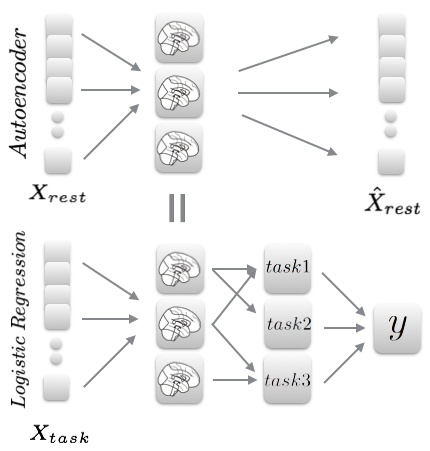
\includegraphics[width=0.40\textwidth]{figures/figure1.png}
  \end{center}
  \caption {\textbf{Architecture}
  }
\end{wrapfigure}

%
\section{Methods}
%
\paragraph{Data.}
Unsupervised projection models into a lower-dimensional space and
supervised logistic-regression models are learned in concert
in a same parameter gradient descent.
Brain
network decompositions are thus exposed that explain task-descriminative spatial
patterns of neural activity.

As the currently biggest openly-accessible reference dataset,
we chose the Human Connectome Project (HCP) for the present analyses
\cite{barch2013}.
Neuroimaging task data with labels of ongoing cognitive processes
were drawn from 500 unrelated,
healthy HCP participants.
18 HCP tasks 
were selected that are known to elicit reliable neural activity
across participants.
The task paradigms include
1) working memory/cognitive control processing, 2)
incentive processing, 3) visual and somatosensory-motor processing,
4) language processing (semantic and phonological processing),
5) social cognition, 6) relational processing, and 7) emotional
processing. All data were acquired on the same Siemens Skyra 3T scanner.
Whole-brain EPI acquisitions were acquired with a
32 channel head coil (TR=720ms, TE=33.1ms, flip angle=52°, BW=2290Hz/Px,
in-plane FOV=$280\times180$mm, 72 slices, 2.0mm isotropic voxels).
The “minimally preprocessed” pipeline includes
gradient unwarping, motion correction, fieldmap-based EPI distortion
correction, brain-boundary-based registration of EPI to structural
T1-weighted scans, non-linear (FNIRT) registration into MNI space,
and grand-mean intensity normalization. Activation maps were spatially
smoothed by a Gaussian kernel of 4mm (FWHM). A GLM was
implemented by FILM from the FSL suite with model regressors from convolution
with a “canonical” hemodynamic response function and from temporal derivatives.
HCP tasks were conceived to modulate activation
in a maximum of different brain regions and neural systems. Indeed, at
least 70\% of the participants showed consistent brain activity in
contrasts from the task battery, which certifies excellent
coverage \cite{barch2013}.
In sum, the HCP task data incorporated 8650 first-level activity maps
from 18 diverse paradigms administered to 498 participants (2 removed
due to incomplete data).
All maps were resampled to a common 60x72x60 space of
3mm isotropic voxels and gray-matter masked (at least 10\% tissue
probability).
All supservised analyses were based on labeled HCP task maps of
79,941 voxels representing Z values in gray matter.

These labeled data were complemented by unlabeled activity maps
from HCP acquisitions of unconstrained resting-state activity.
These reflect brain activity in the absence of controlled thought.
In line with the goal of the present study, acquisition of the data was
specifically aimed at the study of task-rest correspondence.
From each included participant, we included two
time-series for left and right phase encoding
with 1,200 maps of multiband, gradient-echo planar imaging acquired
during a period of 15min (TR=720 ms, TE=33.1 ms, flip angle=52°,
FOV=$280\times180$mm, and 2.0mm isotropic voxels). Besides run duration,
the task acquisitions were identical to the resting-state fMRI acquisitions
for maximal compatibility between task and rest data.
We here drew on ``minimally preprocessed'' rest data
from 200 randomly selected healthy, unrelated participants.
PCA was applied to each set of 1,200 rest maps for
denoising by keeping only the 20 main modes of
variation.
In sum, the HCP rest data concatenated
8000 unlabeled, noise-cleaned rest maps with
40 brain images from each of 200 randomly selected participants.

We were further interested in the utility of the optimal low-rank projection
in one task dataset for dimensionality reduction in another task dataset.
To this end, the HCP-derived network decompositions were used as preliminary
step in the classifcation problem of another large-cohort dataset.
The ARCHI dataset \cite{pinel07} provides activity maps from
diverse experimental tasks, including auditory and visual perception, motor action,
reading, language comprehension and mental calculation.
81 right-handed healthy participants
(3 not included in present analyses due to incomplete data)
without psychiatric or
neurological history participated in four fMRI sessions acquired under
different experimental paradigms.
The functional maps were warped into
the MNI space and resampled to isotropic 3mm resolution.
Whole-brain EPI data were acquired with the same Siemens Trio with a 32
channel head coil (TR=2400ms, TE=30ms, flip angle=60°, in-plane
FOV=$19.2\times19.2$cm, 40 slices, 3.0mm isotropic voxels).
Standard preprocessing was performed with Nipype \cite{gorgo11}, including
slice timing, motion correction, alignment, and spatial normalization.
Activation maps were spatially smoothed by
a Gaussian kernel of 5mm (FWHM).
Analogous to HCP data, the second task dataset incorporated 1404
labeled, grey-matter masked, and z-scored activity maps
from 18 diverse tasks acquired in 78 participants.

\paragraph{Unsupervised layer.}
The labeled and unlabeled data were fed into a linear statistical model.
The model is composed of an autoencoder and a low-rank logistic regression.
On the one hand, the affine autoencoder takes the input 
$x$ and projects it into coordinates of a latent representation $z$
by

\begin{eqnarray}
  \begin{split}
  z &= W_0 x + b_{W_0} \\
  x' &= W_1 z + b_{W_1}
  \end{split}
  \label{eq:autoenc}
\end{eqnarray}

where $x \in \mathbb{R}^{d}$ denotes the vector of $d=79,941$ voxel from each
rest map, $z \in \mathbb{R}^{n}$ is the $n$ hidden dimensions (i.e.,
distributed macroscopical activity patterns), and 
$x' \in \mathbb{R}^{d}$ is the reconstruction vector of the original activity map
from the hidden variables. Further, ${W_0}$ denotes the weight matrix that
transforms
from input space into the hidden space (i.e., encoder),
${W_1}$ is the weight matirx for back-projection from the hidden space to the
output space (i.e., decoder), ${b_{W_0}}$ and ${b_{W_1}}$ are bias vectors.
Note that ${W_0}$ and ${W_1}$ are tied
$W_0$ = $W_1^T$.
The optimal model parameters ${W_0}, {b_{W_0}}, {b_{W_1}}$ are found by
minimizing the reconstruction difference by squared error

\begin{eqnarray}
  {\mathcal{L_{AE}}}(x, x') = || \x - \x' ||^2
\end{eqnarray}

This reconstruction error criterion equates with
maximizing a lower bound on the mutual information between
input and the learned representation.
Non-linearities were not applied on the
transformation results.

\paragraph{Supervised layer.}
On the other hand, such lossy compression by a low-dimensional bottleneck
is also imposed by the first layer of the low-rank
logistic regression.

\begin{eqnarray}
  \begin{split}
    P(Y=i|x, V_0,V_1,b_{V_0}, b_{V_1}) &= softmax_i(V_1 (V_0 x + b_{V_0}) + b_{V_1}) \\
    &= \frac {e^{V_1_i (V_0_i x + b_{V_0}_i) + b_{V_1}_i}} {\sum_j e^{V_1_j (V_0_j x + b_{V_0}_j) + b_{V_1}_j}}            
  \end{split}
  \label{eq:lr}
\end{eqnarray}

\begin{eqnarray}
  \begin{split}
    {\mathcal{L_{LR}}}(x, y) = \sum_{i=0}^{N_{X_{task}}} \log(P(Y=y^{(i)}|x^{(i)}; V_1 (V_0 x + b_{V_0}) + b_{V_1})
\end{split}
\label{eq:lr_loss}
\end{eqnarray}

\begin{wrapfigure}{r}{0.40\textwidth}
  \begin{center}
    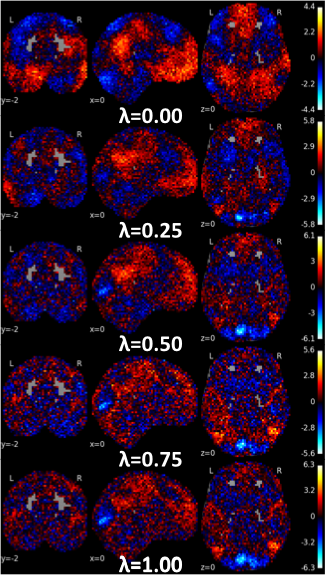
\includegraphics[width=0.40\textwidth]{figures/figure3.png}
  \end{center}
  \caption {\textbf{Equilibrium between autoencoder and low-rank logistic regression}
  One learned decomposition component (out of 20) between the only-autoencoder
  (\textit{uppermost panel}) and only-logistic-regression
  (\textit{lowermost panel}) scenarios.
  The congruent structure (\textit{red, middle column})
  in the
  posterior cingulate cortex, posterior mid-cingulate cortex, and medial
  prefrontal cortex that is hence important in decompositions of the rest and
  task neuroimaging data. With increasing weight on the supervised learning,
  non-congruent structure emerges in the early (\textit{blue}) and
  lateral (\textit{red}) visual cortex
  (\textit{right column}). Matrix weights were z-scored.
  }
\end{wrapfigure}

\paragraph{Layer combination.}
Importantly, the optimization problem of the linear autoencoder
and the low-rank logistic regression
are linked one two levels. First, their transformation matrices mapping from
input to the latent space are identical.
    $V_0 = W_0$
We thus search for a compression of the 79,941 voxel values into $n$ latent
components that represent an optimal encoding for both
rest and task activity data.
Second, the objectives of the autoencoder and the low-rank
logistic regression are combined into a same loss function.

\begin{eqnarray}
  \begin{split}
{arg\,min}_\theta \hspace{0.2cm} {\mathcal{L}}(\theta, \lambda) = \lambda\frac{1}{N_{X_{task}}} {\mathcal{L_{LR}}}
+ (1-\lambda)\frac{1}{N_{X_{rest}}} {\mathcal{L_{AE}}} + \ell_1(\theta) + \ell_2(\theta)
  \label{eq:loss_equ}
\end{split}
\end{eqnarray}

In so doing, we search for the combined set of model parameters
$\theta=\{V_0,V_1,b_{V_0}, b_{V_1}, b_{V_0}, b_{V_1}\}$
with respect to the (unsupervised) reconstruction error and the
(supervised) task classification. For parameter shrinkage, we
impose a combination of \ell_1 and \ell_1 penalties (i.e., elasticnet)
on the parameters \theta.

\paragraph{Optimization.}
The statistical learning problem was approximated in the neuroimaging data
by computing an updating the parameter derivates of the 
semi-supervised low-rank logistic regression.
The required gradients are easily obtained by using the chain rule to
backpropagate error derivatives first through the decoder network
and then through the encoder network 
As solver, we chose \textit{rmsprop} \cite{rmsprop},
a mini-batch version of rprop.
This procedure dictates an adaptive learning rate
for each model parameter by
scaled gradients from a running average.
Gradient normalization by RMSprop
is known to effectively exploit curvature information.
We opted for a small batch size of $100$, given the high degree of
redundancy in $X_{rest}$ and $X_{task}$.
The matrix parameters were initalized by Gaussian random values multiplied
by a gain of $0.004$. The bias parameters were initalized to be zero.
With a slight abuse of notation, let $\theta$ denote a component of $\theta$.
The normalization factor and the update rule for $\theta$
are given by

\begin{eqnarray}
  \begin{split}
v^{(t+1)} &= \rho v^{(t+1)} + (1 - \rho)\left(\frac{\partial f}{\partial \theta}\right)^2
%v^{(t+1)} = \rho v^{(t+1)} + (1 - \rho)˜|\nabla f
\\
\theta^{(t+1)} &= \theta^{(t)} + \alpha \frac{\nabla f(\theta^{(t)})}{\sqrt{v^{(t+1)} + \epsilon}},
  \end{split}
\end{eqnarray}

where $0 < \rho < 1$ constitutes the decay rate. $\rho$ was set to
$0.9$ to deemphasize the magnitude of the gradient.
Further $\alpha$ is the learning rate and $\epsilon$ a global damping factor.
The hyper-parameter $\alpha$ was set to $0.00001$ by prior manuel
cross-validation and $\epsilon$ was set to $1^{-6}$.
%
Note that we have also experimented with other solvers
(stochastic gradient descent, adadelta, and adagrad) but found that
rmsprop converged faster and with higher generalization performance.


\paragraph{Hints.}
In fact, the constraint by a rest-data autoencoder qualifies as a
\textit{hint} rather than regularization \cite{abu1994hints}.
Its purpose is not to prevent overfitting but to introduce
prior knowledge on known properties of the unknown target function $f$.
Rather than relying only on input-output pairs in the learning process,
we thus narrow our hypothesis set to the biologically most plausible solutions.
That is, we reduce the search space in a way that
is compatible with the expected representation of BOLD activity signals.


\paragraph{Implementation.}
The analyses were performed in Python.
We used \textit{nilearn} to handle
the high-dimensional neuroimaging data 
\cite{abrah14}
and
\textit{theano} for automatic
differentiation of symbolic computation graphs
\cite{bastien2012theano, bergstra2010theano}.
All Python scripts that generated the results are
accessible online for reproducibility and reuse
\url{http://github.com/banilo/nips2015}.



\section{Experimental Results}

This was evaluated by the prediction
accuracy on a validation set (20\% of the training data) at each iteration.

all vectors are column vectors

affine encoder and decoder

Low-rank regression outperformed serial ICA/SparsePCA and logistic regression.

reduction of n gray-matter voxels to n components


20 components: high bias/low variance
100 compoentens: low bias/high variance

Generating samples from the learned statistical model



Modifications of the mode that di not improve the genralization performacne:
dropo-out, input corruption, addining non-linearities (sigmoid, tanh),


introducing a
nonlinearity (sigmoid, tanh) into the system did not improve predictive accuracy but
elastic did -> most useful decomposition has characteristics of a SPCA
and not PCA or ICA

outperforms plain vanilla LR
inject prior domain knowledge into the learning process


class weights:
the right model should have high probability in only some places





\section{Discussion and Conclusion}
%
There is an increasing occurrence of high-dimensional problems in the
neuroimaging domain. This calls for new statistical learning algorithms that
behave well in large-cohort settings. Ideally, they should acknowledge
and exploit existing widely-accepted neuroscientific knowledge.
In the present work, we propose such an estimator that learns
dimensionality reduction
in a neurobiologically valid and interpretable fashion.

-hypothesis space includes sparse PCA and PCA but not ICA since no
linearity

respect structure in the fMRI data


- if linearity, then would be closer to the notion of 1-hidden layer neural
network rather than low-rank logistic regression



We hope that these results stimulate the development of
even more powerful semi-supervised classification methods


improve computational tractability, prediction accuracy, and interpretability
neuroimaging datasets
does it produce testable predictions?
-> we can test predictive value of network-network architectures across
mental domains.

open window to study the correspondence between brain dynamics during
every-day mind-wandering and task-focused brain states.

classifier that operates in a (sparse) network space, rather than in a voxel space.
domain-specifc classification algorithms

repertoire of mental operations that the human brain can perform

large quantities of neuroimaging data
logistic regression in an autoencoder paradigm

automatically learn a mapping to and from a brain-network space

statistical structure

PCA:
captures structure in the data that is well described by Gaussian clouds,
linear pair-wise correlations are most important form of statistical
dependence/orthongonal components

-> BOLD images can readily be reduced to linear combinations of
sparse spatial structures

scale different classificatiuon architectures to large neuroimaging data

task data might concentrate near a low-dimensional manifold of brain networks

neurobiolgocial fidelity

entities of the neuroimaging domain

There is much uncertainty about the most pertinent representation
of neural activation information
put probability mas shwere we expeted neurobiological strucuture

canonical set of brain networks


FUTURE
link the restings-tate component to the pattern sof cognitive proceses
reduce information von resting-state data in neurological and psychiatric
populations for discovery of neurobiological sub-groups as well as
prediction of disease trajectories and drug responses


%
\paragraph{Acknowledgment}
{\small
Data were provided the Human Connectome Project. The study was supported
by the German National Academic Foundation (D.B.).
}


\small
\bibliographystyle{splncs03}
\bibliography{nips_refs}

\end{document}
